\documentclass[../../main.tex]{subfiles}

\begin{document}
\providecommand{\diag}{\operatorname{diag}}
\problem{15}
\begin{wts}
Provide a screen shot. 
\end{wts}
\begin{proof}
Consider the following,\\
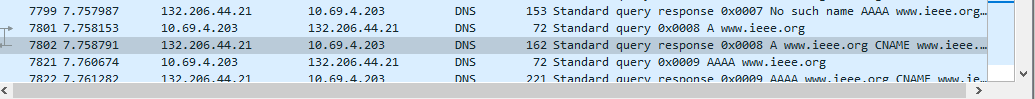
\includegraphics[width=\textwidth]{subfiles/images/308_Lab5_Part_1_PAGE0_1_Image21.png}
\begin{itemize}
    \item class based addressing very bad bad because not flexible
    \item class ABCD too many hosts, or too few hosts,
    \item number of hosts per class?
    \item Class B supports $2^(16)-2 = 65534$ hosts, we subtract 2 from the number of hosts becuase 0.0 is reserved for the network itself, and 255.255 is broadcast.
\end{itemize}
\end{proof}
\begin{proof}
    First let us consider the transmitted signal in Rectangular, 16-QAM. From previous discussions, we have derived the transmitted signal $s(t)$,
    \begin{equation}\label{s(t) form 1} 
    s(t) = 2^{1/2}\biggl(a^I_k\cos(2\pi f_c t)+a^Q_k\cos(2\pi f_c t + \pi/2)\biggr)
    \end{equation}
    and the second form
    \begin{equation}\label{s(t) form 2} 
    s(t) = s_1(t) + s_2(t)
    \end{equation}
    where $s_1(t)$, and $s_2(t)$ are given by
    \begin{align}
        s_1(t) &= 2^{1/2}a_k^I\cos(2\pi f_c t)\label{s_1 equation}\\
        s_2(t) &= 2^{1/2}a_k^Q\cos(2\pi f_c t +\pi/2)\label{s_2 equation}
    \end{align}
    We can isolate $s_1(t)$, the in-phase component by multiplying $s(t)$ with $\cos(\omega t)$, where $\omega = 2\pi f_c$ from here onwards. Without loss of generality,
    \begin{align*}
        s(t)\cos(\omega t)&=2^{1/2}\biggl(a_k^I\cos^2(\omega t) - a_k^Q\sin(\omega t)\cos(\omega t)\biggr)\\
        &=2^{-1/2}\biggl(a_k^I+a_k^I\cos(2\omega t)-a_k^Q\sin(2\omega t)\biggr)
    \end{align*}
    The retrieval of the real-part of the complex symbol $a_k = a_k^I + ja_k^Q$ follows immediately with the application of an ideal low-pass filter. The case, in any AWGN channel holds no surprises too.\\
    
    If $s(t)$ is contaminated with white noise $n(t)$, then it is trivial to verify that the resultant signal, after multiplication and the LPF becomes
    \begin{equation}\label{whitenoise retrieval}
        \operatorname{LPF}\biggl((s(t)+n(t))\cos(\omega t)\biggr)=2^{-1/2}\biggl(a_k^I + \wig{n}(t)\biggr)
    \end{equation}
    From Equation \eqref{whitenoise retrieval}, the demodulation is now an exercise of finding the 'closest' $a\in\mathcal{A}'$ such that
    \[
    \bignorm{\biggl(a_k^I + \wig{n}(t)\biggr)-a}\leq\inf\biggl\{\bignorm{\biggl(a_k^I + \wig{n}(t)\biggr)-a'},\,a'\in\mathcal{A}'\biggr\}
    \]
    for the desired choice of $\norm{\cdot}$. A common way to do this in the 1-D case is to use decision regions, or balls of radius $d/2$, centered around each $a'\in\mathcal{A}'$, where $d = \min\{\norm{x-y},\,x,y\in\mathcal{A}',\,x\neq y\}$. This was the implementation in the Simulink model.
\end{proof}

Applying a low pass filter gets rid of the higher frequency components, and this retrieves the original sine wave spectrum.\\
    
    The reason for why the above works is a simple consequence of the Nyquist sampling theorem. It states that for any bandlimited baseband signal $x(t)$, with bandwidth $T^{-1}/2$, it is enough to sample (multiplication with pulse train) the signal $x(t)$ with a sampling rate of $T^{-1}$ for the full, indistinguishable reconstruction of $x(t)$.\\
    
    The following is a brief summary of the Nyquist sampling theorem, and should suffice for the purposes of this question.
    \begin{itemize}
        \item The pulse train in the time domain is a pulse train in the frequency domain.
        \item Sampling in the time domain $\iff$ multiplication with pulse train.
        \item Sampling in the time domain $\iff$ frequency domain convolution with pulse train.
        \item Sampling creates infinitely many copies of the shifted original spectrum.
        \item As long as you sample at twice the bandwidth of the original signal, there is no aliasing.
        \item Applying a low-pass filter removes the 'copies' of the original spectrum.
    \end{itemize}
    Of course, the ideal low-pass filter is a rectangle in the frequency domain. If $\hat{x}(t)$ sampled $x(t)$, it immediately follows that
    \[
    x(t) = \hat{x}(t)\ast\dfrac{\sin(\pi t/T)}{\pi t/T}
    \]

    \begin{lemma}\label{lemma: diagonal exponential matrix}
    If $D =\diag_{i\leq n}\lambda_i$ is a diagonal matrix, then 
    \[
    e^{Dt} = \diag_{i\leq n}e^{\lambda_i t}
    \]
\end{lemma}
\begin{proof}
    Using the definition of $e^{Dt}$,
    \begin{align*}
        e^{Dt}&= \sum_{k\geq 0} (Dt)^k(k!)^{-1}\\[2ex]
        &=\lim_n\sum^n_{k\geq 0}(Dt)^k(k!)^{-1}\\[2ex]
        &=\lim_n \sum^n_{k\geq 0}\diag_{i\leq n}\biggl( (\lambda_i t)^k(k!)^{-1}\biggr)\\[2ex]
        &=\diag_{i\leq n}\biggl(\lim_n \sum_{k\geq 0}^n (\lambda_it)^k(k!)^{-1}\biggr)\\[2ex]
        &=\diag_{i\leq n}e^{\lambda_i t}
    \end{align*}
\end{proof}
\begin{wts}
    Given a system in state space form as in
    \begin{equation}\label{state space equation q2}
        \dot{x} = Ax + Bu
    \end{equation}
    Alternatively in the time domain
    \begin{equation}\label{state space equation q2 time domain}
        x(t) = e^{At}x_0 + \int_0^t e^{A(t-\alpha)}Bu(\alpha)d\alpha,\: t\geq 0
    \end{equation}
    If there exists some $u(t)$ such that $x(T) = x_f$ for any fixed $x(0) = x_0$, then we claim if that another LTI system, $(\cl{A}, \cl{B}, \cl{C}, \cl{D}, \cl{x}, \cl{y}, \cl{u})$ satisfies
    \begin{enumroman}
        \item $\cl{A} = -A$,\label{q2 param1}
        \item $\cl{B} = -B$,\label{q2 param2}
        \item If $\cl{x}_0 = x_f$, and\label{q2 param3}
        \item given the input $\cl{u}(t)=u(T-t)$ on $[0, T]$\label{q2 param4}
    \end{enumroman}
    We will have $\cl{x}(T) = \cl{x}_f= x_0$ In other words, this LTI system 'reverses' steering.
\end{wts}
\begin{proof}
    Substitute $t = T$ within \eqref{state space equation q2 time domain}, and solving for $x_0 = \cl{x}_f$. Noting that $e^{At}$ is invertible at every $t\geq 0$ with inverse $(e^{At})^{-1} = e^{(-A)t}$
    \[
        x(T) = e^{AT}x_0 + \int^T_0 e^{A(T-\alpha)}Bu(\alpha)d\alpha
    \]
    Isolating $x_0$, and swapping $T-\alpha$ with $\alpha$ in the convolution integral,
    \[
    x_0 = e^{(-A)T}x(T) - e^{(-A)T}\int^T_0 e^{A\alpha}Bu(T-\alpha)d\alpha
    \]
    Since we want $\cl{x}_f = x_0 = \cl{x}(T)$
    \begin{align*}
        \cl{x}(T) = e^{(-A)T}\cl{x}_0 + \int^{T}_0 e^{-A(T-\alpha)}(-B)u(T-\alpha)d\alpha
    \end{align*}
    Now substitute the values within \ref{q2 param1}, \ref{q2 param2}, \ref{q2 param3}, and \ref{q2 param4}, we have
    \[
    \cl{x}_f = e^{\cl{A}T}\cl{x}_0 + \int^{T}_0 e^{\cl{A}(T-\alpha)}\cl{B}\cl{u}(T-\alpha)d\alpha
    \]
    This completes the proof.

\end{proof}

\end{document}